\chapter*{Introduction}\label{ch:introduction}
\addcontentsline{toc}{section}{\nameref{ch:introduction}}
Mobile communication systems have over the past two decades, become a foundation for modern society. Communication has always been a fundamental necessity for human society, but the recent years have indeed shown how great of an engineering achievement cellular networks are. The mobile phone has evolved into a device that enables an enormous amount of services. For most people, what goes on behind the scenes of a mobile phone is considered black magic. Most people do not question it as long as it just \emph{works}. However, when it does not work, or \emph{no service} is displayed, the annoyance is more significant than anything. Regardless of the annoyance level reached, these mobile communication services are paramount to modern society. If not only for entertainment but also for essential emergency communication services. As technology evolves, so does mobile communication systems. The development and on-going process of deploying \gls{nr} solutions is the foundation for a multitude of communication services. The capabilities of \gls{nr} are many, one of which is the expected industrial revolution where automatization is in focus. However, first and foremost, to offer increased capacity and coverage. The increased capacity, lower latency and improved energy efficiency are vital properties of \gls{nr}-based networks. These improved capabilities are driven not only by demand but also by necessity. 

\gls{ai} have in recent years been shown to be capable of solving complex problems surpassing human performance in tasks such as image recognition or language translation. These performances have not gone unnoticed and have attracted incredible attention from mainstream media. The models behind these advances are in broad strokes identified by \acrfull{dl}. While modern mobile communication systems may be an incredible feat of engineering, it is still faced with many complex problems of management and optimization. The recent advances in \acrlong{dl} coupled with the increased demand and solutions for mobile communication, sparked the PhD project behind this dissertation. Current mobile communication systems are advanced, sophisticated, and any additions must be selected with patience and deliberation. The adaptability of \acrlong{dl} has been hailed as an essential part in overcoming these problems and a key enabler for future mobile networks. This dissertation seeks to explore the role and feasibility of \gls{ai} solutions in current and future mobile communication systems through novel applications. 

The main limitation of mobile communication networks is the transmission of information over the air using radio waves. The radio environment in mobile communication systems is difficult to characterize due to many complex interactions on both a macroscopic and microscopic level. The fundamental theoretical understanding of radio propagation has been established and can offer insight into this complex and dynamic environment; however, at the cost of extreme computational complexity. To ensure reliable transmission in the current mobile systems, it requires an enormous amount of so-called channel state information. This information is to ensure the right actions are taken when transmitting to and from a user. This amount of information is significant. So significant that it in practice is capable of storing $2^{24}$ channel coefficients per millisecond per operating base station \cite{Studer2018}. The base station is the entity that connects to mobile devices present in the environment. Data quantity is the main driver for \acrlong{dl}-solutions.  By formalizing problems as learning objectives, \acrlong{dl} can be used to obtain correlation, information and insight from otherwise insensible data. The data quantities of the radio environment, coupled with the requirements for \acrlong{dl} defines the areas of contributions within this dissertation.


\section*{Areas of contribution}
The focus of the contributions within this dissertation is on the so-called \emph{physical layer} of mobile communication systems, seen in Fig. \ref{fig:areas_of_contribution}. For any communication system, this layer is associated with the practicalities of transmitting and receiving the raw information over the transmission medium. In the case of mobile communication systems, the transmission medium is foremost considered \emph{the air}. 


\begin{figure*}
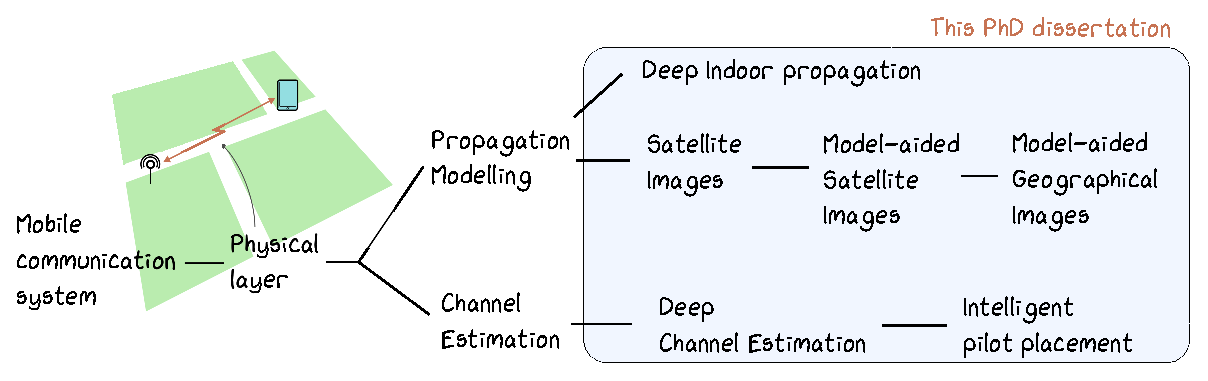
\includegraphics[width=\textwidth]{chapters/figures/intro_figure.eps}
\caption{Contributions of this dissertation}\label{fig:areas_of_contribution}
\end{figure*}

\section*{Contributions}

The contributions of this dissertation can be reduced to the following specific items. 

\begin{itemize}
    \item Chapter \ref{ch:channelmodellingbasics}, A provided Ray-tracing model for mobile communication systems offer no performance improvements compared to existing empirical models.
    \item Chapter \ref{ch:satelliteImages}, Deep Learning can significantly improve path loss estimation for unseen locations.
    \item Chapter \ref{ch:satelliteImages}, Geographical Images contain information useful for path loss prediction that can be extracted with supervised learning.
    \item Chapter \ref{ch:deepindoor}, Deep-indoor propagation characteristic is shown to be determined by a complex combination of geo-statistical features.
    \item Chapter \ref{ch:deepindoor}, Deep Learning is identified as an essential tool for engineering features used for modelling deep-indoor propagation.
    \item Chapter \ref{ch:channel_estimation}, Channel estimation in uplink transmission can significantly be improved by using Deep Learning.
    \item Chapter \ref{ch:channel_q_learning}, Deep Reinforcement Learning can enable autonomous solutions for designing optimum pilot placement in uplink.
\end{itemize}

\noindent Specifically, the above have been formalized into peer-review published research papers. The list of associated research papers can be found below.


\section*{Paper contributions}

The asterisk \emph{*} denotes research papers awaiting peer-review. They can be found in Appendix \ref{app:submitted_papers}.

\vspace{2em}

\noindent \textbf{Thrane, J.} \&  Artuso, M. \&  Zibar, D. \&  Christiansen, H. L. (2018). \textit{Drive Test Minimization Using Deep Learning with Bayesian Approximation}. 2018 IEEE 88th Vehicular Technology Conference (VTC-Fall) \cite{Thrane2018DriveApproximation}

\vspace{2em}


\noindent Artuso, M. \&  \textbf{Thrane, J.} \&  Christiansen, H. L. (2018). \textit{User-Centric Power Saving in Self-Organizing Mobile Networks.} 2018 IEEE 88th Vehicular Technology Conference (VTC-Fall) \cite{Artuso2018User-CentricNetworks}

\vspace{2em}

\noindent \textbf{Thrane, J.} \&  Zibar, D. \&  Christiansen, H. L. (2019). \textit{Comparison of Empirical and Ray-Tracing Models for Mobile Communication Systems at 2.6 GHz}. 2019 IEEE 90th Vehicular Technology Conference (VTC2019-Fall) \cite{Thrane2019ComparisonGHz}

\vspace{2em}

\noindent \textbf{Thrane, J.} \&  M., Zibar, D. \&  Christiansen, H. L. \textit{Model-aided Deep Learning Method for Path Loss Prediction in Mobile Communication Systems at 2.6 GHz}. IEEE Access 2020 \cite{Thrane020ModelAidedDeepLearning}

\vspace{2em}

\noindent \textbf{Thrane, J.} \&  Christiansen, H. L. \textit{Pilot Placement Method for Future Cellular Systems in Uplink at 2 GHz using Deep Q-Learning}. IEEE OJVT 2020, submitted \cite{Thrane2020PilotQ-Learning} *


\vspace{2em}

\noindent \textbf{Thrane, J.} \&  Sliwa, B. \& Wietfeld, C. \& Christiansen, H. L. \textit{Deep Learning-based Signal Strength Prediction Using Geographical Images and Expert Knowledge}. IEEE Globecom 2020, submitted \cite{Thrane2020DeepKnowledge} *

\vspace{2em}
\noindent 
Ruepp S. \& Mateo A. C.  \& Malarski K. M.  \& \textbf{Thrane J.}  \&  Petersen, M. N. (2018). \textit{Internet of Things Connectivity in Deep-Indoor Environments}. 2018 9th International Conference on the Network of the Future \cite{Malarski2018DemonstrationCases}

\vspace{2em}
\noindent Malarski, K. M. \& \textbf{Thrane, J.} \&  Bech, M. G. \&  Macheta, K. \&  Christiansen, H. L.  \& Petersen  M. N. \& Ruepp  S. \textit{Investigation of deep indoor NB-IoT propagation attenuation}. IEEE 90th Vehicular Technology Conference 2019 Fall (VTC2019-Fall) \cite{Malarski2019InvestigationAttenuation}

\vspace{2em}
\noindent \textbf{Thrane, J.} \&  Malarski, K. M. \& Christiansen, H. L. \& Ruepp, S. \textit{Experimental Evaluation of Empirical NB-IoT Propagation Modelling in a Deep-Indoor Scenario}. IEEE Globecom 2020, submitted \cite{Thrane2020ExperimentalScenario} *


\section*{Dataset contributions}

\noindent \textbf{Thrane, J.} \& Christiansen, H. L. \textit{Mobile Communication System Measurements and Satellite Images}. IEEE DataPort 2019 \cite{1xf4-eg98-19}

\vspace{2em}
\noindent \textbf{Thrane, J.} \& Christiansen, H.L. \& Bech, M. G. \textit{Technical University of Denmark LTE drive test measurements} IEEE DataPort 2020 \cite{keyt-8g44-20}

\section*{Implementation contributions}

\noindent \textbf{Thrane, J.} \textit{GitHub repository for the dissertation: Optimization of Mobile Communication Systems using Deep Learning}. GitHub 2020 \cite{Thrane2020RepositoryLearning}.


\section*{Dissertation structure}
 
The dissertation is structured into three separate parts. 

\paragraph{Part I} In chapter \ref{ch:monster} an introduction to the state of mobile communication systems and optimizations hereof is given along. Along with this, a motivation for \gls{ml}-based solutions is given. Additionally, in chapter \ref{ch:mlbasics} a brief introduction to \gls{ml} is provided along with short descriptions of the most important \gls{ml} terms used for the remainder of the dissertation. 

\paragraph{Part II} In chapter \ref{ch:channelmodellingbasics} introduces traditional means of modelling the wireless channel. This includes a focus on an empirical and ray-tracing model. A comparison study of the traditional models are presented, discussed and concluded. Chapter \ref{ch:satelliteImages} contains a novel methodology for estimating signal quality metrics for unseen locations in mobile communication systems utilizing geographical images. The method is evaluated and improved over several iterations; the finding of each iteration is presented. Chapter \ref{ch:deepindoor} contains the study of wireless transmission in a deep-indoor situation, utilizing \gls{nbiot} terminology. The results of a comprehensive measurement campaign are presented along with an identified direction for \gls{ml}-based solutions.  The findings of applying \gls{dl} for radio propagation modelling is summarized and discussed in chapter \ref{ch:dl_radio_summary}.

\paragraph{Part III} In chapter \ref{ch:pilot_sequence} so-called pilot signals for current cellular systems are introduced. The current and future issues of so-called \emph{pilot contamination} is introduced along with a discussion of existing solutions found in the literature. In chapter \ref{ch:channel_estimation} a novel method for channel estimation is presented. The results and challenges of the method are discussed in detail. In chapter \ref{ch:channel_q_learning}, a reinforcement learning method for combating pilot contamination and improving channel estimation is presented. Finally, the challenges associated with \gls{ml}-based solutions for channel estimation and pilot optimization are discussed. 

\paragraph{Part IV} In chapter \ref{ch:contributions} an overview of the contributions offered by this dissertation is given. The contributions are discussed in detail, and a perspective to practical considerations is given. Additionally, the challenges identified throughout the dissertation are summarized. A discussion of \gls{dl}-based solutions in mobile communication systems is given. Finally, in chapter \ref{ch:conclusion} a conclusion is provided.




